\pdfoutput=1
\documentclass[11pt]{article}
\usepackage{ACL2023}
\usepackage{times}
\usepackage{latexsym}
\usepackage[T1]{fontenc}
\usepackage[utf8]{inputenc}
\usepackage{microtype}
\usepackage{inconsolata}
\usepackage{booktabs}
\usepackage{amsmath}
\usepackage{placeins}
\usepackage{graphicx}
\usepackage{stfloats}

\begin{document}
\begin{titlepage}
    \begin{center}
        \vspace*{\fill}
        {\Huge\bfseries Revenue Growth as a Predictor of Stock Price Movements \par}
        \vspace{0.3cm}
        {\LARGE\bfseries Evidence from U.S. Public Companies \par}
        \vspace{2.5cm}
        {\Large\bfseries Authors \par}
        \vspace{1cm}
        {\large
        Maya Aharon \par
        \texttt{mayaaharon1@mail.tau.ac.il} \par
        ID: 324126630 \par
        \vspace{0.5cm}
        Ohad Shushan \par
        \texttt{ohadshushan@mail.tau.ac.il} \par
        ID: 211719711 \par
        \vspace{0.5cm}
        Itay Ebenspanger \par
        \texttt{ebenspanger@mail.tau.ac.il} \par
        ID: 322532698 \par
        \vspace{0.5cm}
        Almog Tavor \par
        \texttt{almogt@mail.tau.ac.il} \par
        ID: 323084962 \par
        }
        \vspace{2cm}
        {\Large Tel Aviv University \par}
        {\large August 2025 \par}
        \vspace*{\fill}
    \end{center}
    \thispagestyle{empty}
\end{titlepage}

\begin{abstract}
We examine whether revenue growth serves as a predictor of future stock price movements for U.S. public companies. Using quarterly financial data from over 5,000 firms spanning 2020–2024, we test the relationship between year-over-year revenue growth and forward-looking stock price changes across multiple time horizons (6 months to 3 years). While initially investigating free cash flow growth, we find revenue growth demonstrates superior predictive power.

To answer this, we apply least squares regression with resistance standard errors, controlling for outliers and grouping firms by size and index inclusion. We compare revenue and cash flow metrics across horizons and market segments.

The results reveal a consistent, statistically significant positive relationship between revenue growth and future returns, especially for large-cap and index-listed firms. However, explanatory power remains modest ($R^2$ typically below 0.1), limiting standalone investment applications.

These findings suggest revenue growth carries meaningful predictive information, though best used as part of a broader, multi-factor approach.
\end{abstract}

%introduction
\section{Introduction}

The relationship between corporate financial metrics and stock price movements has been a central question in finance for decades. While the efficient market hypothesis suggests that publicly available information should be quickly incorporated into stock prices, substantial empirical evidence indicates that fundamental analysis can provide insights into future price movements, particularly over medium to long-term horizons.

In this study we ask the question: \textbf{Does revenue growth serves as a reliable predictor of future stock price changes across different market capitalization tiers and time horizons?}

Revenue reflects a company's overall business performance and is often seen as a leading indicator of future profitability. Unlike metrics such as earnings or free cash flow, it is less affected by accounting adjustments, offering a clearer view of underlying fundamentals.

In our research, we examined the relationship between revenue growth and future stock performance through several complementary analyses. First, we conducted a comparison between revenue growth and free cash flow growth as predictors of stock returns, finding that revenue metrics show a clear advantage. Second, we analyzed differences in predictive power across market capitalization tiers, revealing that mega-cap stocks display much stronger fundamental-price relationships. Third, we investigated how inclusion in major indices (S\&P 500, NASDAQ-100, Dow Jones 30) influences these relationships. Finally, we compiled and made publicly available a comprehensive dataset \citep{cash-time-machine-dataset} and the full analysis code \citep{cash-time-machine-code}, enabling replication and further exploration of our findings.

Using data from U.S. public companies between 2020 and 2024, we apply least squares regression with resistance standard errors to examine how year-over-year revenue growth relates to future stock price changes over different time horizons. We control for outliers by trimming extreme values and account for differences between companies by grouping them into market capitalization tiers.

\subsection{Data Collection and Preparation}

We built a dataset of quarterly financial statements and daily stock prices for over 5,000 U.S. public companies from 2020 to 2024. We used two primary data sources: SimFin's API \citep{simfin} for financial data in 2020-2023, and Yahoo Finance accessed through the yfinance Python library \citep{yfinance} for data in 2024-2025 to ensure currency and completeness.

For each company, revenue and stock price growth were calculated as the percentage change from the report date to the corresponding date in subsequent periods (6 months, 1 year, 2 years, and 3 years ahead).

\subsection{Data Quality and Limitations} 

Our dataset exhibits survivorship bias, as delisted companies disappear from current price feeds. We handle missing values and infinite growth rates (from zero-revenue base periods) through resistance outlier detection, trimming observations beyond the 3rd-97th percentiles for micro-caps, 1.5th–98.5th for mega/mid-caps and all samples, and 0.5th–99.5th for index-only analyses.

\begin{table*}[!htbp]
  \setlength{\tabcolsep}{4pt}
  \centering
\caption{Sample rows from our dataset illustrating the relationship between revenue growth and stock price movements for AMZN (2021-2023) and GOOG (Q3-Q4 2021). The full dataset spans thousands of U.S. stocks over multiple quarters, all in USD.}
  \label{tab:sample-data}
  \begin{tabular}{lccrrrr}
    \toprule
    Ticker & Report Date & Price & 1Y Price Growth & Market Cap (bn) & Revenue (bn) & 1Y Revenue Growth \\
    \midrule
    AMZN & 2021-12-31 & 166.72 & 2.38\%   & 1,683.87 & 469.822 &  21.70\% \\
    AMZN & 2022-12-31 &  85.82 & -48.52\% &   876.22 & 513.983 &   9.40\% \\
    AMZN & 2023-12-31 & 149.93 & 74.70\%  & 1,538.19 & 574.785 &  11.83\% \\
    \midrule
    GOOG & 2021-09-30 & 132.47 & 81.37\%  & 1,763.86 & 65.118 &   41.02\% \\
    GOOG & 2021-12-31 & 143.82 & 65.18\%  & 1,884.32 & 75.325 &   32.35\% \\
    \bottomrule
  \end{tabular}
\end{table*}

%methodology
\section{Methodology}

\subsection{Initial Approach: Free Cash Flow Analysis}

We initially hypothesized that free cash flow (FCF) growth would serve as a strong predictor of future stock price movements, given its representation of a company's fundamental ability to generate excess cash. FCF was calculated as operating cash flow minus capital expenditures, normalized by shares outstanding to obtain FCF per share growth rates.

However, our preliminary analysis revealed extremely weak relationships across all market capitalization tiers. For the 1Y horizon, FCF growth showed virtually no explanatory power: $R^2 = 0.000$ for all samples, with Pearson correlations ranging from 0.003 (mid-caps) to 0.040 (mega-caps). Even for mega-caps at longer horizons, the maximum $R^2$ achieved was only 0.029 (3-year), indicating FCF growth alone provides insufficient predictive power for stock price movements.

\subsection{Transition to Revenue Growth Analysis}

Given the poor performance of FCF-based metrics, we pivoted to revenue growth as our primary explanatory variable. Revenue represents the top-line fundamental driver of corporate value and tends to be less volatile than bottom-line metrics like FCF, which can be affected by timing of capital investments and accounting treatments.

\subsection{Statistical Framework}

We use least squares regression with resistance standard errors, modeling the relationship:

\begin{equation}
\textit{PriceGrowth}_{i,t+h} = a + b \cdot \textit{RevenueGrowth}_{i,t} + \epsilon_{i,t}
\end{equation}

where $i$ indexes firms, $t$ indexes quarterly report periods, and $h$ represents forward-looking horizons (6M, 1Y, 2Y, 3Y). We implement outlier control by trimming observations beyond the 3rd and 97th percentiles for both dependent and independent variables.

To account for differences between companies, we group them by market capitalization tier:
\begin{itemize}
\item \textbf{Micro-caps}: Bottom 10\% by market cap
\item \textbf{Mid-caps}: Middle 80\% by market cap  
\item \textbf{Mega-caps}: Top 10\% by market cap
\end{itemize}

We also analyze specific market indices (S\&P 500, NASDAQ-100, Dow Jones 30) to examine whether index inclusion affects the revenue-price relationship.

\subsection{Hypothesis Testing}

Our analysis focuses on examining whether there is a linear relationship between revenue growth and future price growth. This is reflected in three steps:  
\\ 1. Conducting hypothesis tests, where we test \( H_0: b = 0 \) against \( H_1: b \neq 0 \) using t-tests with resistance standard errors.
\\ 2. Calculating the Pearson correlation coefficient and the coefficient of determination (\(R^2\)) to measure the strength and direction of the relationship. We also examine the least squares regression line (minimizing the residual sum of squares, RSS) as well as the resistance regression line, and report the corresponding p-values.
\\ 3. Computing 95\% confidence intervals for the estimated coefficients.

The analysis assumes a linear relationship between the variables, independence of observations (except for repeated observations of the same company), and homoscedasticity after applying resistance standard errors. Coefficients are estimated using the Least Squares method, and statistical significance is evaluated at the 0.05 level.

%results
\section{Results}

\subsection{Statistical Significance of $b_{LS}$ Estimates}

In all regressions, we tested the null hypothesis $H_0: b_{LS} = 0$ and evaluated statistical significance using a standard t-test. Across all horizons, subsamples, and index-based splits, the p-values are consistently below the conventional threshold of 0.05 (in most cases, well below $<0.001$), leading us to \textbf{reject the null hypothesis in every single case}. This indicates that the Least Squares estimator return coefficient is statistically significant throughout the entire analysis.

\subsubsection{Insights from Main Sample by Horizon and Size}

Table~\ref{tab:regression-all} summarizes regression outcomes across four horizons (6M, 1Y, 2Y, 3Y), and by size tier (All, Mega, Micro, Mid caps).

Key findings include:

\begin{itemize}
    \item The $b_{LS}$ coefficient is consistently positive and statistically significant across all tiers and time horizons, with stronger magnitudes in longer horizons. For example, the highest values of $b_{LS} = 0.4352$ are observed for Mega-caps at both 1Y and 2Y horizons, with corresponding p-values $<0.001$.
    
    \item The $R^2$ values indicate moderate explanatory power, especially for Mega-caps and longer horizons (peaking at $R^2 = 0.086$ for Mega-caps at 3Y), with highly significant p-values (e.g., $<0.001$). The low p-values support the explanatory strength of the model.

    \item Pearson correlation values also increase with horizon length, and are highest for Mega-caps (e.g., Pearson = 0.293 at 3Y), indicating stronger linear relationships in larger-cap samples, accompanied by highly significant t-statistics and p-values below 0.001.

    \item While all results lead to rejection of $H_0$, the \textbf{strongest signal} appears in the 1Y and 2Y horizons for Mega-caps. This is due to the relatively high $b_{LS}$ values, high Pearson correlations, and very low p-values, suggesting that return predictability is most pronounced in these segments.
\end{itemize}

Figure~\ref{fig:revenue-by-cap} shows regression results across all stocks (post-clipping), linking revenue growth over time frame $h$ from time $t$ to stock returns in the period $[t+h,\ t+2h]$, for $h \in {6\text{M},\ 1\text{Y},\ 2\text{Y},\ 3\text{Y}}$.
In every case, the least-squares slope $b_{LS}$ is positive and highly significant ($p<0.001$), so we reject $H_0\colon b=0$ at the 5\% level.
Although modest - ranging from 1.4\% at 6 months to 2.7\% at 1 year - $R^2$ consistently exceeds zero, indicating revenue growth captures a small but reliable part of price variation.
Splitting by market cap reveals a clear hierarchy: mega-caps show the strongest fit (e.g.\ $b_{LS}=0.4352$, $R^2=8.1\%$ at 1 year), mid are intermediate, and micro-caps are weakest ($b_{LS}\approx0.018$-0.062, $R^2\le1.2\%$).
Resistance line slopes are even higher, confirming robustness to outliers after basic clipping of 3\% we did in both sides in micro-caps vs.\ 1.5\% elsewhere.
Despite significance, the low $R^2$ reflects external influences like news and sentiment.
Mega-caps likely benefit from higher coverage, while micro-caps are the most unstable due to events like bankruptcies or buyouts, sometimes showing thousands of percentages of price swings.
Based on thousands of stock-report observations, we selected the 1-year revenue and return window, which consistently showed the strongest results (for all samples, $b_{LS}$ of $0.188$, $R^2$ of $0.027$, $SE$ of $0.005$ and Pearson correlation of $0.165$).

\subsubsection{Insights from Index-Based 1Y Horizon}

Table~\ref{tab:regression-1y-index} focuses on 1Y horizon regressions, segmented by major U.S. indices: S\&P 500, NASDAQ-100, and Dow Jones 30. This breakdown was chosen due to the relatively high correlation observed at the 1Y horizon in the main sample.

Key findings include:

\begin{itemize}
    \item All three index-based samples yield statistically significant $b_{LS}$ coefficients, with p-values well below 0.001, and again the null hypothesis is rejected in all cases.

    \item The NASDAQ-100 and Dow Jones 30 exhibit particularly strong results:
        \begin{itemize}
            \item NASDAQ-100 has the highest $b_{LS} = 0.6957$ and Pearson correlation of 0.339, with p-value $<0.001$.
            \item Dow Jones 30 shows the highest $R^2 = 0.230$ and Pearson correlation of 0.480, despite its smaller sample size, and with a highly significant p-value $<0.001$. This suggests strong statistical confidence in the observed relationship.
        \end{itemize}

    \item Compared to the 1Y results in Table~\ref{tab:regression-all}, these index-specific samples, especially Dow Jones 30, demonstrate stronger relationships. This suggests that in more concentrated or higher-quality indices, return predictability may be more pronounced, supported by large effect sizes and extremely low p-values.
\end{itemize}

Figures~\ref{fig:sp500},\ref{fig:nasdaq100}, and\ref{fig:dow30} illustrate the relationship between 1Y revenue growth and stock price change across the S\&P 500, NASDAQ-100, and Dow Jones 30. Each plot includes both the Least Squares (LS) regression line and the Resistance Line (RL), visually supporting the statistical analysis in Table~\ref{tab:regression-1y-index}. All three indices show a positive linear trend, with varying strength: S\&P 500 presents a moderate signal ($b_{LS}=0.354$, $R^2=0.071$, Pearson = 0.266), NASDAQ-100 shows the steepest slope and stronger sensitivity to revenue growth ($b_{LS}=0.696$, $R^2=0.115$, Pearson = 0.339), while Dow Jones 30 demonstrates the most consistent relationship overall, with the highest explanatory power and correlation ($b_{LS}=0.614$, $R^2=0.230$, Pearson = 0.480). In all cases, the Resistance Line ($b_{RL}$) is flatter than $b_{LS}$, reflecting adjustment for outliers. These visuals reinforce our core finding: revenue growth is more predictive of future returns in large, mature, and well-followed firms, especially those in concentrated, high-quality indices.

\FloatBarrier

\subsubsection{Confidence Intervals by Market Cap and Horizon}

Figure~\ref{fig:confidence-intervals} displays 95\% confidence intervals for the LS slope ($b_{LS}$) across market cap tiers and time horizons. Mega-cap stocks show the highest and most statistically significant slopes across all horizons, especially at 1Y and 2Y, with intervals clearly above zero. Mid-caps exhibit moderate slopes with tighter intervals, while micro-caps have weaker, noisier estimates with wider intervals, often near zero. Overall, the predictive power of revenue growth is strongest for large firms and over medium-term horizons, aligning with earlier regression findings.

\FloatBarrier

\begin{table*}[!htbp]
\centering
\caption{Regression Results for Main Sample Across All Horizons}
\label{tab:regression-all}
\small
\begin{tabular}{lcccccccccc}
\toprule
Horizon & Tier & N & $b_{LS}$ & $R^2$ & $b_{RL}$ & p-value & t-stat & t-crit & SE & Pearson \\
\midrule
6M  & All Samples & 45217 & 0.1149 & 0.014 & -0.062 & <0.001 & 25.753 & 1.960 & 0.00446 & 0.120 \\
6M  & Mega-caps   & 4537  & 0.2226 & 0.034 &  0.010 & <0.001  & 12.565 & 1.960 & 0.0177  & 0.183 \\
6M  & Micro-caps  & 4288  & 0.0617 & 0.007 & -0.054 & <0.001    &  5.374 & 1.961 & 0.0115  & 0.082 \\
6M  & Mid-caps    & 36171 & 0.1293 & 0.017 & -0.056 & <0.001 & 24.880 & 1.960 & 0.0052  & 0.130 \\
\midrule
1Y  & All Samples & 39991 & 0.1875 & 0.027 & -0.157 & <0.001 & 33.462 & 1.960 & 0.0056  & 0.165 \\
1Y  & Mega-caps   & 3983  & 0.4352 & 0.081 & -0.004 & <0.001  & 18.774 & 1.961 & 0.0232  & 0.285 \\
1Y  & Micro-caps  & 3764  & 0.0952 & 0.012 & -0.062 & <0.001  &  6.840 & 1.961 & 0.0139  & 0.111 \\
1Y  & Mid-caps    & 31762 & 0.1979 & 0.028 & -0.126 & <0.001 & 30.289 & 1.960 & 0.00653 & 0.168 \\
\midrule
2Y  & All Samples & 29433 & 0.1265 & 0.023 & -0.180 & <0.001 & 26.263 & 1.960 & 0.00482 & 0.151 \\
2Y  & Mega-caps   & 2950  & 0.4352 & 0.085 &  0.050 & <0.001  & 16.555 & 1.961 & 0.0263  & 0.292 \\
2Y  & Micro-caps  & 2740  & 0.0459 & 0.009 & -0.283 & <0.001   &  4.918 & 1.961 & 0.00933 & 0.094 \\
2Y  & Mid-caps    & 23588 & 0.1321 & 0.024 & -0.126 & <0.001 & 23.942 & 1.960 & 0.00552 & 0.154 \\
\midrule
3Y  & All Samples & 20149 & 0.0932 & 0.017 & -0.302 & <0.001  & 18.508 & 1.960 & 0.00504 & 0.129 \\
3Y  & Mega-caps   & 2021  & 0.3910 & 0.086 &  0.043 & <0.001  & 13.774 & 1.961 & 0.0284  & 0.293 \\
3Y  & Micro-caps  & 1883  & 0.0178 & 0.003 & -0.324 & 0.0209                  &  2.311 & 1.961 & 0.00772 & 0.053 \\
3Y  & Mid-caps    & 16129 & 0.1024 & 0.019 & -0.196 & <0.001  & 17.711 & 1.960 & 0.00578 & 0.138 \\
\bottomrule
\end{tabular}
\end{table*}
\begin{table*}[!htbp]
\centering
\caption{Regression Results for 1Y Horizon (Index-Specific Samples)}
\label{tab:regression-1y-index}
\small
\begin{tabular}{lcccccccccc}
\toprule
Index & N & $b_{LS}$ & $R^2$ & $b_{RL}$ & p-value & t-stat & t-crit & SE & Pearson \\
\midrule
S\&P 500     & 7253 & 0.3536 & 0.071 & -0.105 & <0.001 & 23.508 & 1.960 & 0.0150 & 0.266 \\
NASDAQ-100   & 1549 & 0.6957 & 0.115 &  0.104 & <0.001  & 14.170 & 1.961 & 0.0491 & 0.339 \\
Dow Jones 30 &  430 & 0.6140 & 0.230 &  0.157 & <0.001 & 11.312 & 1.966 & 0.0543 & 0.480 \\
\bottomrule
\end{tabular}
\end{table*}

\begin{figure*}[!htbp]
\centering
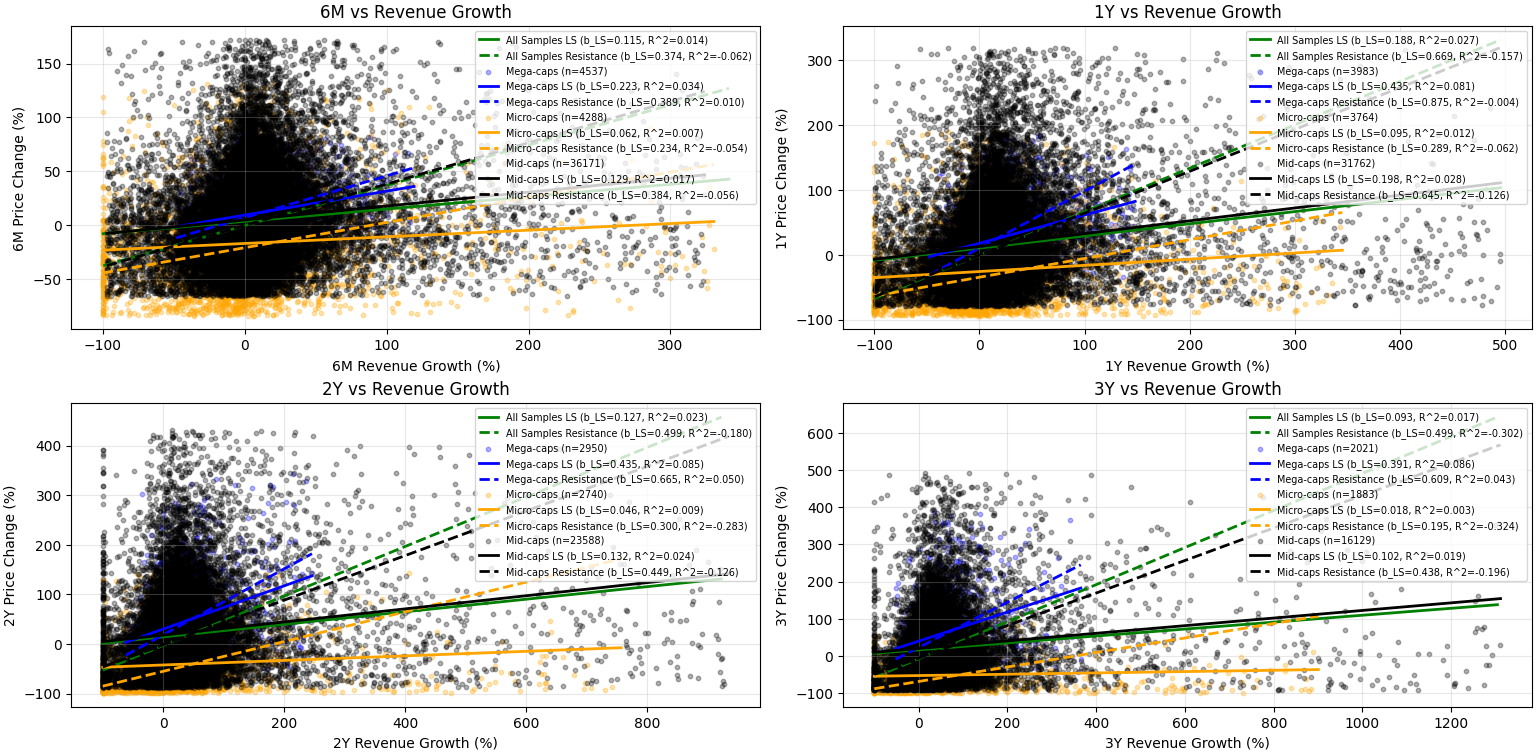
\includegraphics[width=\textwidth]{images/all_horizons_all_stocks_single_plot.png}
\caption{Revenue growth vs. price changes across time horizons (6M, 1Y, 2Y, 3Y) and market cap tiers. Mega-caps show the strongest relationships, followed by micro-caps and mid-caps.}
\label{fig:revenue-by-cap}
\end{figure*}
\begin{figure*}[!htbp]
\centering
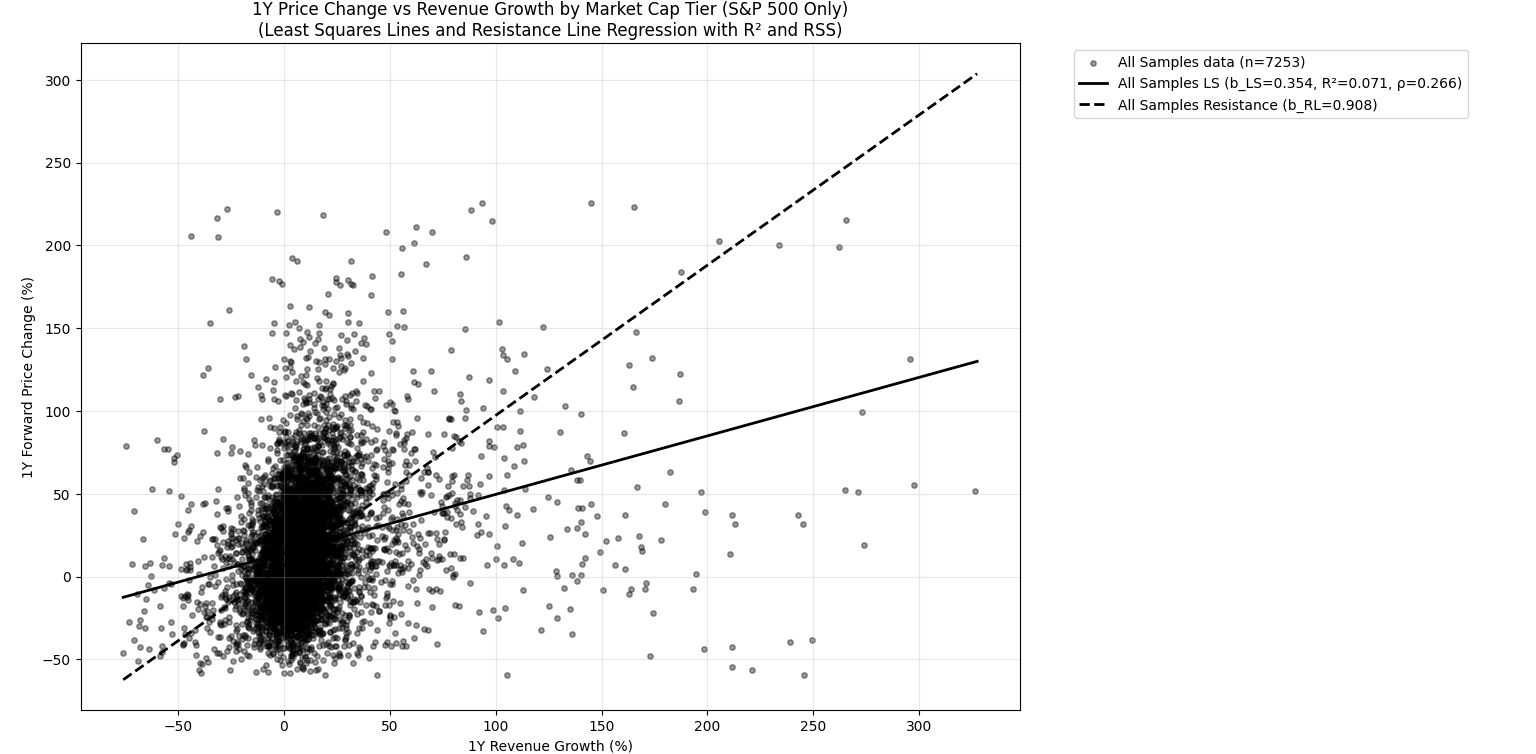
\includegraphics[width=\textwidth]{images/1_year_sp500_plot.png}
\caption{S\&P 500 constituents: 1Y price change vs. revenue growth. Index constituents show stronger fundamental-price relationships than the broader market.}
\label{fig:sp500}
\end{figure*}

\begin{figure*}[!htbp]
\centering
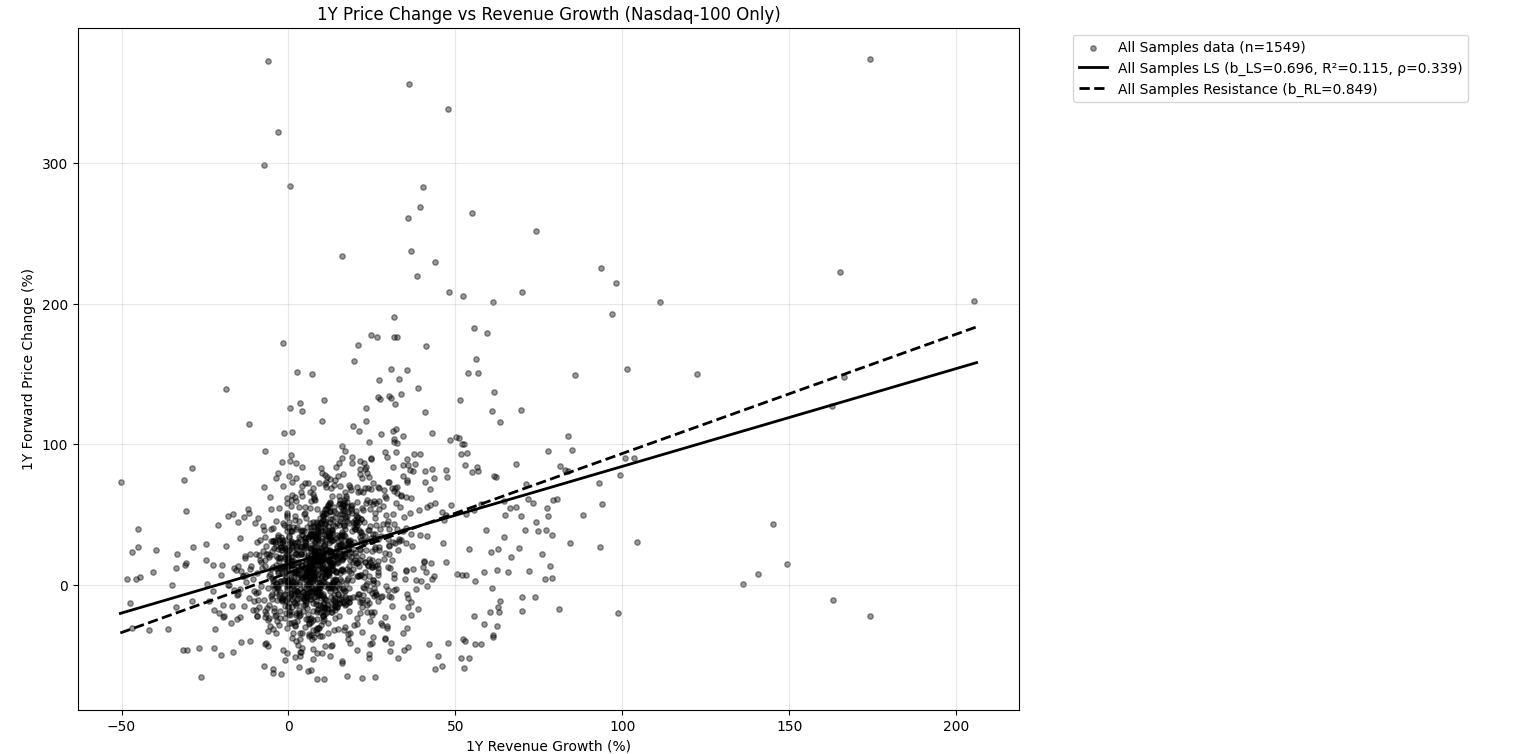
\includegraphics[width=\textwidth]{images/1_year_nasdaq100_plot.png}
\caption{NASDAQ-100 constituents: 1Y price change vs. revenue growth. Technology-focused index shows robust revenue-price relationships.}
\label{fig:nasdaq100}
\end{figure*}

\begin{figure*}[!htbp]
\centering
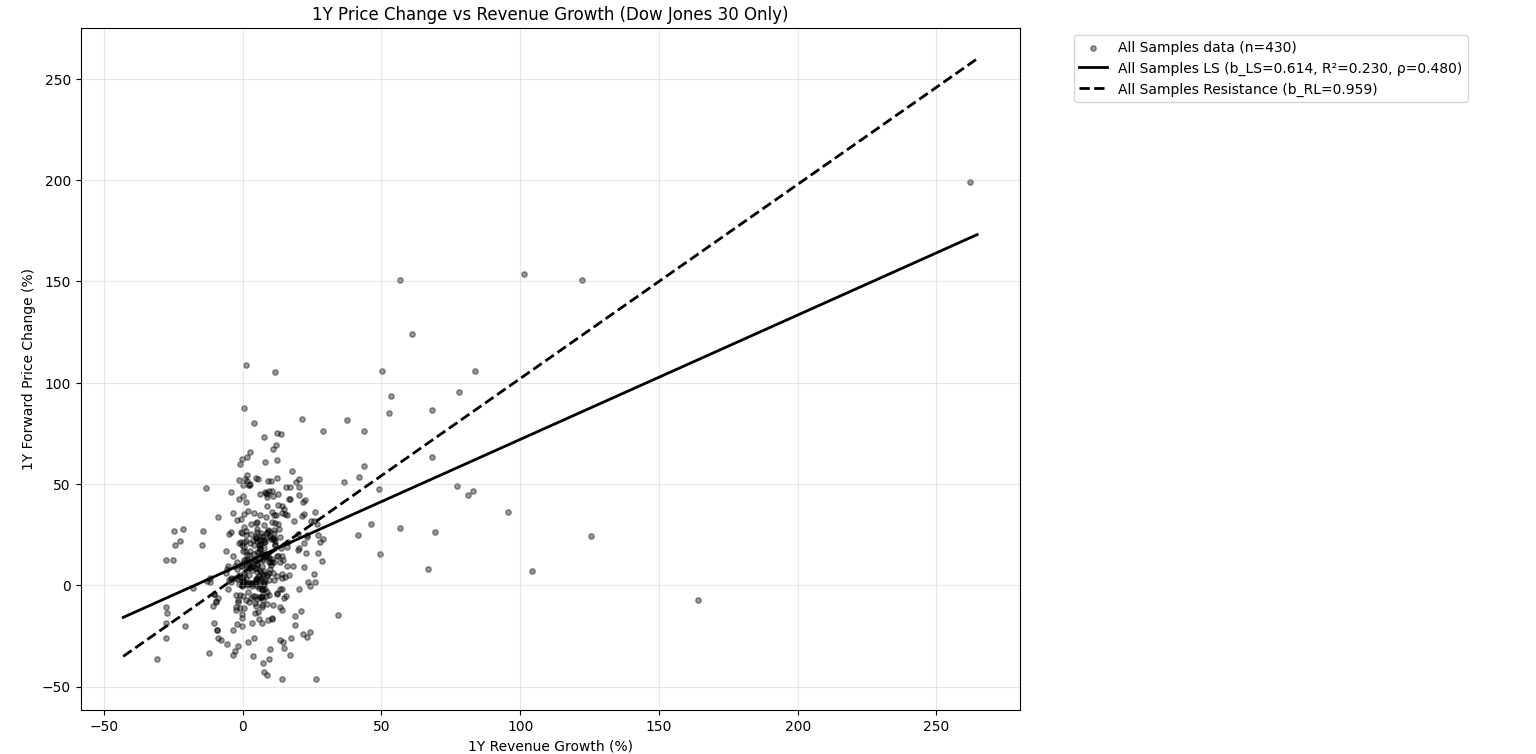
\includegraphics[width=\textwidth]{images/1_year_dow30_plot.png}
\caption{Dow Jones 30 constituents: 1Y price change vs. revenue growth. Blue-chip stocks demonstrate strong fundamental-based pricing relationships.}
\label{fig:dow30}
\end{figure*}
\begin{figure*}[!htbp]
\centering
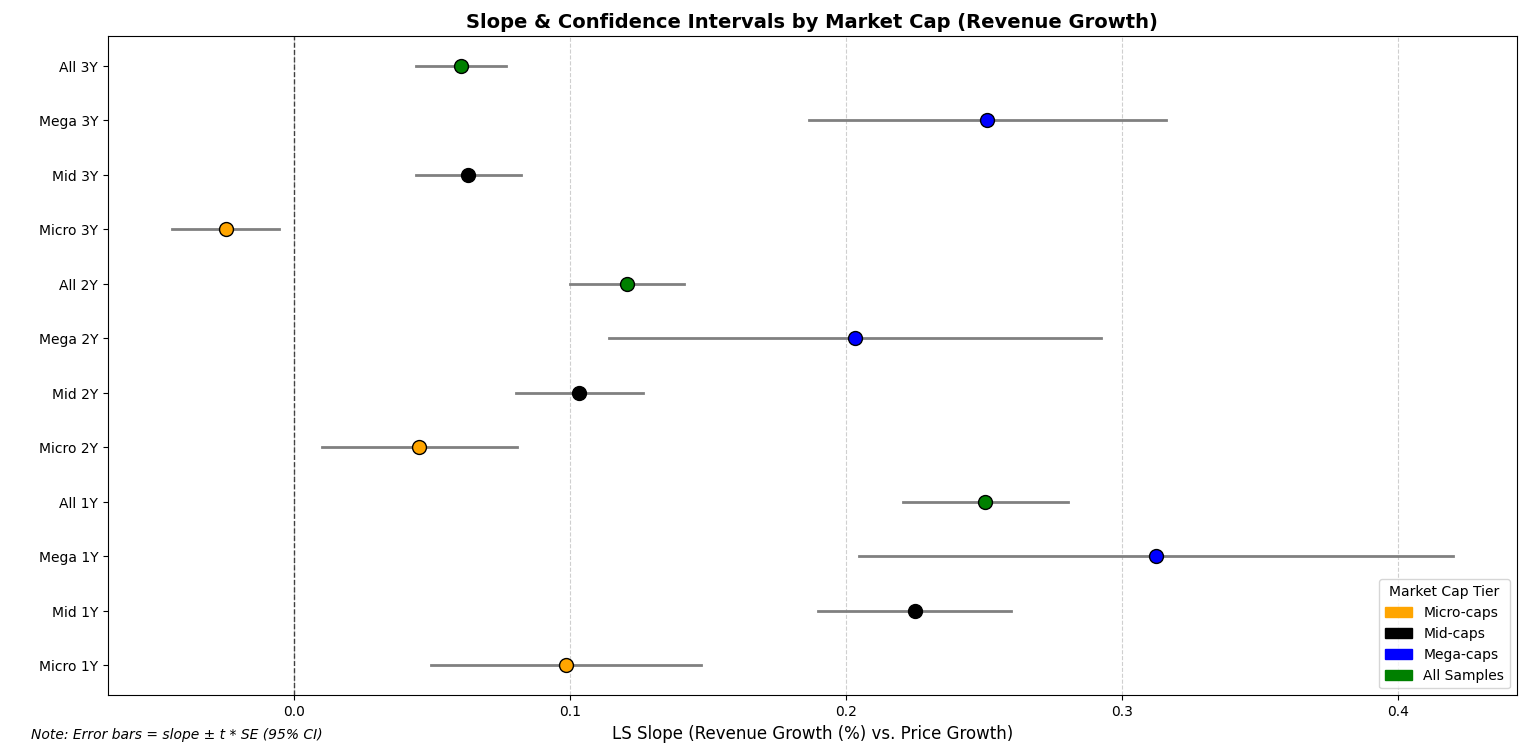
\includegraphics[width=\textwidth]{images/all_horizons_confidence_intervals.png}
\caption{95\% confidence intervals for slope coefficients across market cap tiers and time horizons. Error bars show standard errors for least squares estimates.}
\label{fig:confidence-intervals}
\end{figure*}

%discussion and conclusions
\section{Discussion and Conclusions}

In this project, we examined whether revenue growth can predict future stock price movements, using data from over 5,000 U.S. public companies. We were motivated by our shared interest in stocks and the financial markets, and wanted to better understand how company fundamentals relate to future stock performance.

The analysis confirms that revenue growth holds predictive value, particularly for large-cap and index-listed firms. The relationship is stronger over medium-term horizons and in companies with greater transparency and investor attention. This suggests that revenue, as a top-line indicator, is priced more efficiently in mature, high-quality firms.

While the models' explanatory power is limited, as expected in financial forecasting, revenue growth emerges as a useful signal when interpreted in context. The confidence intervals support the robustness of the findings, especially for large firms.

Our analysis is limited by survivorship bias, missing key variables such as profitability and industry effects, and a relatively short time frame. While results are statistically significant, the low explanatory power limits their standalone use in investment decisions without broader context or risk management.

To summarize, we ran a script that measured the top stocks by revenue growth from Q2 of 2024 to 2025, in order to identify the most compelling stock opportunities for our current year (2025 to 2026), based on our model, Table~\ref{tab:top-winners} highlights the top 3 predicted winners across all groups.
These stocks show the highest forecasted price increases based on their recent revenue growth.

Notably, NVIDIA (NVDA) ranks first in the mega-cap group with a predicted gain of 54.3\%, followed by Eli Lilly (LLY) and ServiceNow (NOW), both showing strong fundamentals and high statistical confidence (t-stat = 7.77). These companies stand out not only for their strong revenue expansion but also because the model assigns them a relatively high predictive significance. 

\begin{table}[!htbp]
\centering
\caption{Top 3 Predicted Winners Based on Revenue Growth (Q2 2024 onward)}
\label{tab:top-winners}
\begin{tabular}{lcccccc}
\toprule
Rank & Ticker & Market Cap & Quarter & Revenue Growth & Predicted Gain & t-stat \\
\midrule
1 & NVDA & \$2656.1B & Q2 2025 & 69.2\% & 54.3\% & 7.77 \\
2 & LLY  & \$739.9B  & Q1 2025 & 45.2\% & 43.1\% & 7.77 \\
3 & NOW  & \$213.3B  & Q2 2025 & 22.4\% & 32.5\% & 7.77 \\
\bottomrule
\end{tabular}
\end{table}

\section{Data and Code Availability}

To facilitate replication and further research, we have open-sourced both our complete dataset and analysis code. The dataset, containing quarterly financial statements and daily stock prices for over 5,000 U.S. public companies from 2020-2025, is available on HuggingFace Datasets \citep{cash-time-machine-dataset}. The full analysis code, including data collection, processing, and statistical modeling scripts, is available on GitHub \citep{cash-time-machine-code}.

\FloatBarrier

\bibliography{anthology,custom}
\bibliographystyle{acl_natbib}

\end{document}